\section{Zielsetzung}
Das Ziel dieses Versuches ist es das Elastizitätsmodul verschiedener Metalle zu bestimmen.

\section{Theorie}
\label{sec:Theorie}

Wenn Kräfte an Oberflächen von Körpern angreifen, können diese Gestalts- und Volumenveränderungen hervorrufen.
Diese Kräfte bezogen auf die Flächeneinheit heißt Spannung.
Die senkrecht zur Oberflächen verlaufende Komponente heißt Normalspannung $\sigma$ und die parallele Komponente wird Tangentialspannung genannt.
Die Formänderung kann durch die relative Änderung $\sfrac{\delta L }{L}$, mit einer linearen Körperdimension $L$, beschreiben werden.
Ist diese Änderung hinreichend klein, entsteht eine lineare Beziehung zwischen $\sfrac{\delta L }{L}$ und der Spannung $\sigma$.
Diese Beziehung heißt das Hookesche Gesezt und hat die Form
\begin{equation}
    \sigma = E \frac{\delta L}{L}
\end{equation}
Hierbei ist $E$ das Elastizitätsmodul, welches eine Materialkonstante ist.
Um diese zu bestimmen, wird eine spezielle Deformation verwendet, die sogenannte Biegung.
\subsection{Durchbiegung eines homogenen Stabes bei einseitiger Einspannung}
\begin{figure}
    \centering
    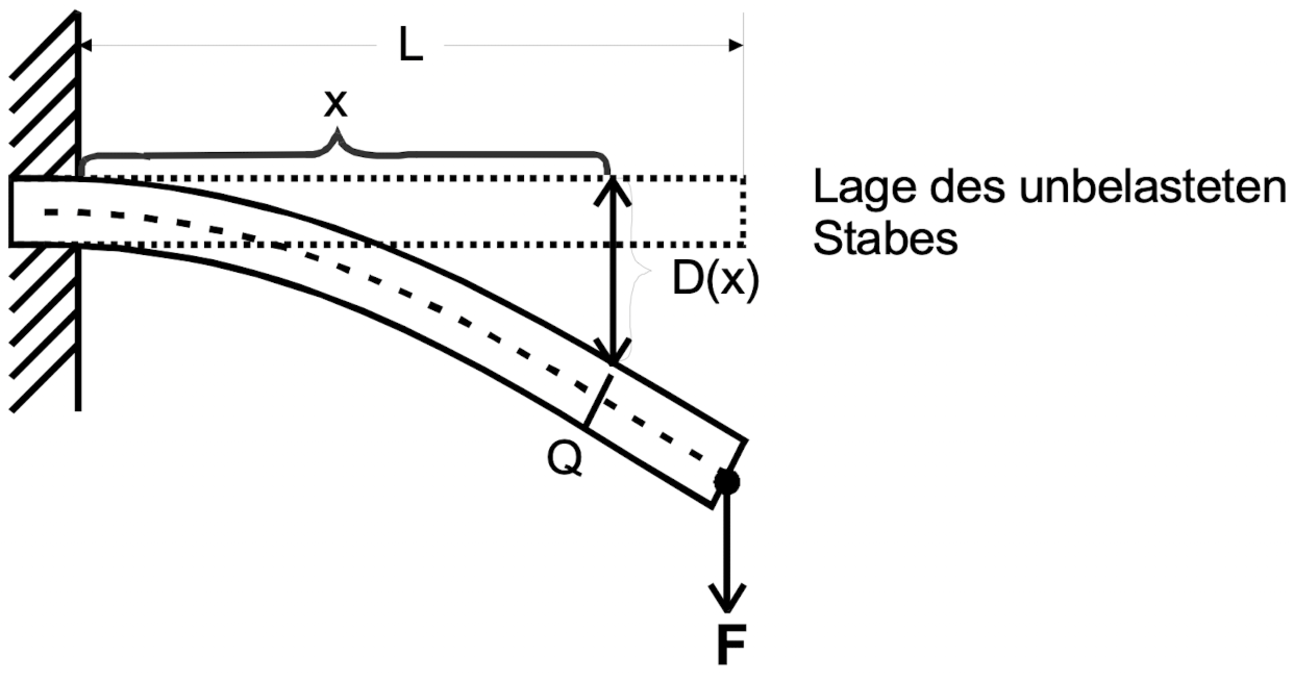
\includegraphics[height=3.5cm]{Abbildungen/einseitige_Einspannung.pdf}
    \caption{Durchbiegung eines elastischen Stabes bei einseitiger Einspannung}
    \label{fig:einseitige_Einspannung}
\end{figure}
Der Versuchsaufbau ist in \autoref{fig:einseitige_Einspannung} dargestellt.
Es soll die Durchbiegung $D(x)$, also die Verschiebung eines Oberflächenpunktes $x$ zwischen belastet und unbelastet errechent werden.
Mithilfe von $D$ lässt sich mit den gemessenen Größen $E$ bestimmen.
Wie in \autoref{fig:einseitige_Einspannung} zu sehen, wird der Querschnitt $Q$ aus seiner vertikalen Lage durch die Kraft $F$ verdreht.
Auf ihn wirkt das Drehmoment $M_\text{F}$.
Auf die obere Schicht des Stabes wirkt die Zugspannung, somit wird sie gedehnt.
Auf die untere Schicht dagegen wirkt die Drucksapnnung und sie wird gestaucht.
Die Schicht dazwischen wird weder gedehnt, noch gestaucht.
Diese wird als neutrale Faser bezeichnet und ist in \autoref{fig:einseitige_Einspannung} als gestrichelte Linie dargestellt.
\begin{figure}
    \centering
    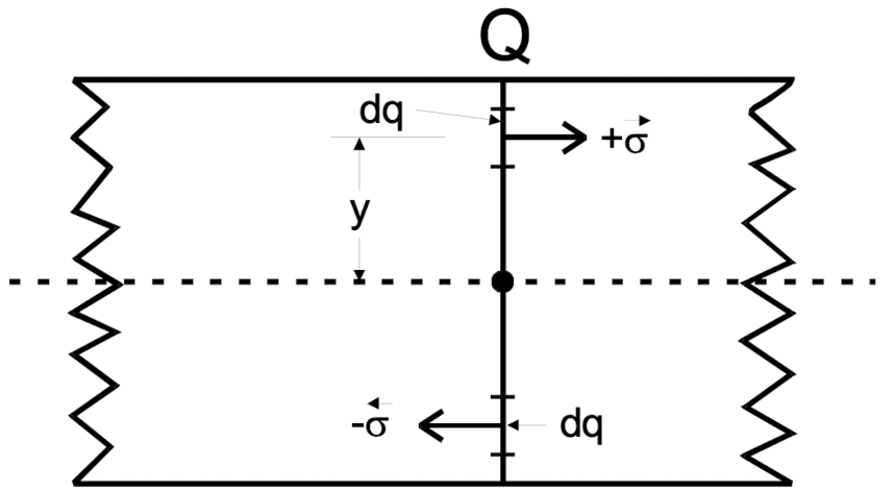
\includegraphics[height=3.5cm]{Abbildungen/Skizze_Drehmoment.pdf}
    \caption{Skizze zur Berechnung des Drehmoments $M_\sigma$}
    \label{fig:Drehmoment}
\end{figure}
In \autoref{fig:Drehmoment} ist die Richtung der Zug- und Druckspannung in dem Stab dargestellt.
Diese zeigen in entgegengesetzte Richtungen und bewirken somit ein Drehmoment $M_\text{\sigma}$.
Durch ein sich einstellendes Gleichgewicht, können die beiden Drehmomente $M_\text{F}$ und $M_\text{\sigma}$ gleichgesetzt werden.
Es ergibt sich
\begin{align*}
    M_\text{F} &= M_\text{\sigma} \\
    F(L-x) &= \int_{Q} y \sigma(y) dq  \, .
\end{align*}
Mit den Hookschen Gesetz ergibt sich für ein kurzes Stabstück der Länge $\Delta x$ und dem Abstand $y$ 
von der neutralen Faser die Normalspannung
\begin{equation*}
    \sigma (y) = E \frac{\delta x}{\Delta x} \, .
\end{equation*}
\begin{figure}
    \centering
    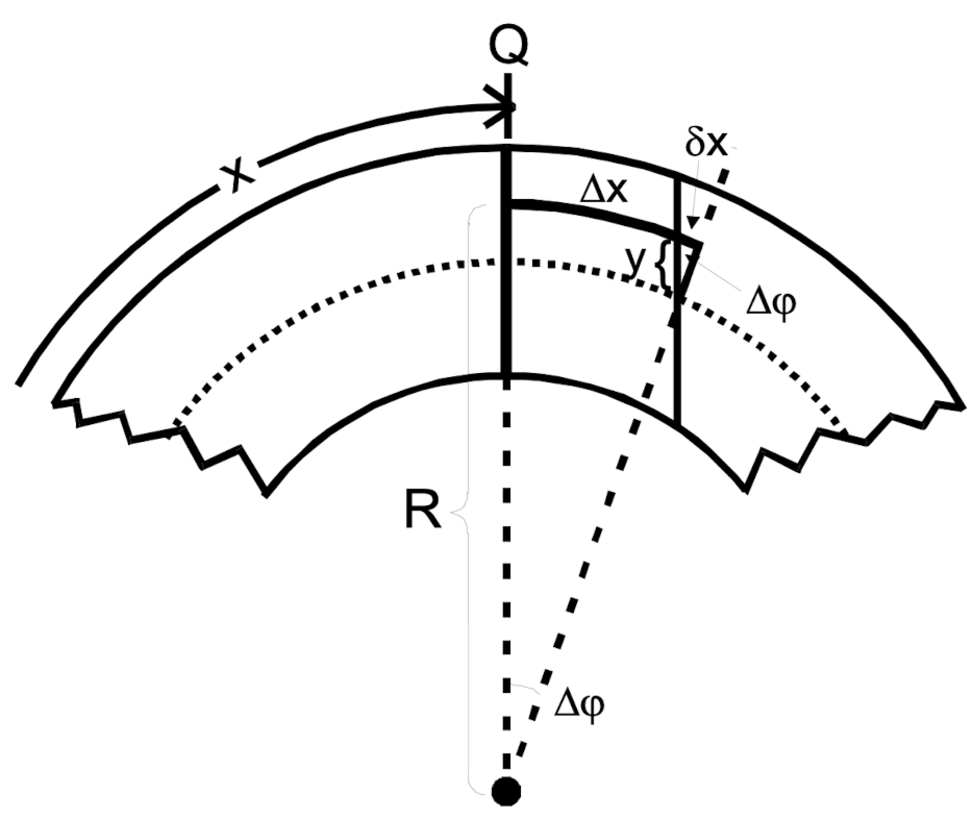
\includegraphics[height=3.5cm]{Abbildungen/Skizze_Normalspannung.pdf}
    \caption{Skizze zur Berechnung der Normalspannung $\sigma (y)$ in einem gebogenen Stab}
    \label{fig:Normalspannung}
\end{figure}
Mit den geometrischen Überlegungen in \autoref{fig:Normalspannung}
und unter der Voraussetzung, dass es sich um geringe Kurvenkrümmungen handelt, folgt
\begin{equation} \label{eq:DGL}
    E \frac{d^2 D}{d x^2} I = F(L-x) \, .
\end{equation}
Hierbei ist $I$ das Flächenträgheitsmoment, welches sich mit
\begin{equation}
    I = \int_{Q} y^2 dq(y)
\end{equation}
berechnet.
Nach Lösen von \autoref{eq:DGL} folgt für die einseitige Einspannung
\begin{equation}
    D(x) = \frac{F}{2EI}(Lx^2-\frac{x^3}{3}) \, \, \, (für 0 \leq x \leq L) \, .
\end{equation}

\subsection{Durchbiegung eines homogenen Stabes bei zweiseitiger Auflage}
Ist der Stab an seinen beiden Enden aufgelegt, und eine Kraft greift in der Mitte an, wirkt die Kraft
$\sfrac{F}{2}$ an $Q$.
Somit verändert sich $M_\text{F}$ zu
\begin{align*}
    M_\text{F} & = - \frac{F}{2} x &\text{für} &\, \,0 \leq x \leq L/2 \\
    M_\text{F} & = - \frac{F}{2} (L -x) &\text{für} &\, \,L/2 \leq x \leq L \, .
\end{align*}
Somit änder sich $D(x)$ zu
\begin{align}
    D(x) & = \frac{F}{48EI}(3L^2x-4x^3) & \text{für} &\, \,0 \leq x \leq \frac{L}{2} \\
    D(x) & = \frac{F}{48EI}(4x^3- 12Lx^2+9L^2x-L^3) & \text{für} &\, \, \frac{L}{2} \leq x \leq L \, .
\end{align}

\subsection{Zusammenhang zwischen Elasitizitätsmodul und Schallgeschwindigkeit in Festkörpern}
Eine andere Methode zur Bestimmung des Elastizitätsmoduls geschieht mithilfe der Schallgeschwindigkeit.
Die Schallgeschwindigkeit in einem Festkörper steht in einfachem Zusammenhang mit dessen Elastizitätsmodul.
Diese Methode ist besonders geeignet, da die Messung nicht durch das Phänomen der elastischen Nachwirkung beeinflusst wird.
Wenn eine longitudinal Welle durch den Körper geht, erzeugt diese eine Spannung $\sigma (x)$.
Da das Hookesche Gesezt hier gelten muss, kann mithilfe von diesem eine Differenzialgleichung aufgestellt werden,
dessen Lösungen allen Gleichungen der Form $f(x \pm ct)$ sind.
Um die Differenzialgleichung zu erfüllen, muss
\begin{equation}
    c = \sqrt {\frac{E}{\rho}}
\end{equation}
sein.
$c$ ist hierbei die gesuchte Fortpflanzungsgeschwindigkeit der elastischen Deformation durch den Schall.
